En este capítulo hablaré sobre los diferentes niveles de optimización que se pueden seleccionar durante la compilación y sus consecuencias en el programa final. Para ver dichas consecuencias se propondrá un programa que se ejecute en la placa microcontroladora y con el que se podrán medir los efectos de las optimizaciones. Por último se creará un programa que muestra las limitaciones de la biblioteca Arduino y que, además, está relacionado con las telecomunicaciones.
\section{Niveles de optimización}
Durante la compilación es posible especificar, mediante la opción \orden{-O} diferentes niveles de optimización. Estos niveles agrupan una serie de optimizaciones.

\begin{table}[htb]
\begin{center}
\begin{tabularx}{\textwidth}{lX}
    \textbf{Nivel de optimización} & \textbf{Descripción}\\
    \hline
   	\orden{-O0} & Opción por defecto. Reduce el tiempo de compilación y facilita la depuración.\\
    \orden{-O1} & Optimiza, pero aumenta el tiempo de compilación y la memoria empleada.\\
    \orden{-O2} & Optimiza más todavía. \programa{GCC} realiza casi todas la optimizaciones que no impliquen aumento del tamaño del programa.\\
    \orden{-O3} & Optimiza todavía más que \orden{-O2}, incluyendo las optimizaciones que aumenten el tamaño del ejecutable.\\
    \orden{-Os} & Optimiza el tamaño del programa. Habilita todas las optimizaciones de \orden{-O2} que normalmente no aumenten el tamaño del código y realiza más optimizaciones destinadas a reducir el tamaño del programa.\\
  \end{tabularx}
\end{center}
\caption{Niveles de optimización}
\label{tab:optimizacionx}
\end{table}

Cada uno de estos niveles (a excepción de \orden{-Os}) añade una serie de optimizaciones sobre el nivel inicial \orden{-O0}.

Para poder averiguar qué optimizaciones lleva acabo el compilador dependiendo del nivel podemos emplear la órden \orden{pic32-gcc -Ox -Q --help=optimizers | grep enabled}, sustituyendo \orden{x} por el nivel que queramos. Esta orden muestra todas las posibles optimizaciones, indicando si están habilitadas o no; y para ver solo las habilitadas pasamos el resultado a \orden{grep}, para filtrarlas.

\begin{table}[htb]
\begin{center}
	\begin{tabular}{ll}
		-falign-loops & -fargument-alias\\
		-fbranch-count-reg & -fcommon\\
		-fdata-sections & -fdce\\
		-fdelete-null-pointer-checks & -fdse\\
		-fearly-inlining & -fgcse-lm\\
		-finline-functions-called-once & -fivopts\\
		-fjump-tables & -fmath-errno\\
		-fmove-loop-invariants & -fpeephole\\
		-frename-registers & -fsched-critical-path-heuristic\\
		-fsched-dep-count-heuristic & -fsched-group-heurisitc\\
		-fsched-interblock & -fsched-last-insn-heuristic\\
		-fsched-spec & -fsched-spec-insn-heuristic\\
		-fsched-stalled-insns-dep & -fsigned-zeros\\
		-fsplit-ivs-in-unroller & -ftoplevel-reorder\\
		-ftrapping-math & -ftree-cselim\\
		-ftree-forwprop & -ftree-loop-im\\
		-ftree-loop-ivcanon & -ftree-loop-optimize\\
		-ftree-phiprop & -ftree-pta\\
		-ftree-reassoc & -ftree-scev-cprop\\
		-ftree-slp-vectorize & -ftree-vect-loop-version\\
		-funit-at-a-time & -fvar-tracking\\
		-fvar-tracking-assignments & -fweb\\
	\end{tabular}
\end{center}
\caption{Optimizaciones del nivel 0.}
\label{opt0}
\end{table}

Como se puede apreciar en la figura~\ref{opt0}, en el nivel más bajo, \programa{gcc} ya realiza optimizaciones. Todas las optimizaciones que comienzan con \orden{-ftree} afectan al árbol sintáctico que utiliza \programa{gcc} como representación interna del programa. También se puede observar cómo una de las optimizaciones que incluye este nivel es \orden{-fdata-sections} y, a pesar de esto, \programa{MPIDE} la incluye explícitamente cuando ejecuta la compilación. Otro grupo de optimizaciones que ya aparecen en este nivel son las que comienzan \orden{-fsched}, que afectan a la reordenación de instrucciones (en ensamblador) para aprovechar lo mejor posible la segmentación de instrucciones del procesador evitando ciclos de espera. En este nivel, si el programa tiene una función que solo es llamada una vez, su llamada será sustituida por el contenido de la función, directamente, gracias a la opción \orden{-finline-functions-called-once}.

\begin{table}[htb]
\begin{center}
	\begin{tabular}{ll}
		-fcprop-registers & -fdefer-pop\\
		-fdelayed-branch & -fforward-propagate\\
		-fguess-branch-probability &-fif-conversion\\
		-fif-conversion2 & -fipa-pure-const\\
		-fipa-reference & -fmerge-constants\\
		-fomit-frame-pointer & -fsplit-wide-types\\
		-ftree-ccp & -ftree-ch\\
		-ftree-copy-prop & -ftree-copyrename\\
		-ftree-dce & -ftree-dominator-opts\\
		-ftree-dse & -ftree-fre\\
		-ftree-sink & -ftree-sra\\
		-ftree-ter & \\
	\end{tabular}
\end{center}
\caption{Optimizaciones que añade el nivel `O1' al nivel `O0'.}
\label{opt1}
\end{table}

En el nivel 1 se añaden más optimizaciones que afectan al arbol sintáctico (Tabla~\ref{opt1}), suponiendo estas casi la mitad de las nuevas optimizaciones. \orden{-fif-conversion} y \orden{-fif-conversion2} tienen como obejtivo tratar de transformar secciones de código donde se usan saltos condicionales para que no los requieran, reduciendo de esta forma el número de instrucciones. También encontramos aquí \orden{-fdelayed-branch}, que intentará reordenar las instrucciones para aprovechar el tiempo que se pierde durante saltos condicionales. Si se produce una instrucción de salto condicional, no es posible saber cúal es la instrucción que se debe ejecutar después, hasta que acabe; por lo que, normalmente, la siguiente instrucción suele ser un \orden{nop}. Si el procesador lo soporta, se mueve una de las instrucciones anteriores a la instrucción de salto que no tenga ninguna dependencia con esta, para aprovechar el hueco libre. En lugar de colocar después del salto una instrucción anterior, \programa{gcc} también trata de predecir, con la opción \orden{-fguess-branch-probability}, que se ejecutará después, por lo que este lugar lo ocupará la primera instrucción de uno de los destinos. Si la predicción resulta errónea, se descartará esta instrucción.

\begin{table}[htb]
\begin{center}
	\begin{tabular}{ll}
		-falign-functions & -falign-jumps\\
		-falign-labels & -fcaller-saves\\
		-fcrossjumping & -fcse-follow-jumps\\
		-fexpensive-optimizations & -fgcse\\
		-finline-small-functions & -fipa-cp\\
		-fipa-sra & -foptimize-register-move\\
		-foptimize-sibling-calls & -fpeephole2\\
		-fregmove & -fremove-local-statics\\
		-freorder-blocks & -freorder-functions\\
		-frerun-cse-after-loop & -fschedule-insns\\
		-fschedule-insns2 & -fstrict-aliasing\\
		-fthread-jumps & -ftree-builtin-call-dce\\
		-ftree-pre & -ftree-switch-conversion\\
		-ftree-vrp & \\
	\end{tabular}
\end{center}
\caption{Optimizaciones que añade el nivel `O2' al nivel `O1'.}
\label{opt2}
\end{table}

El nivel 2 incluye muchas más optimizaciones (Tabla~\ref{opt2}). En este nivel encontramos las optimizaciones \orden{-falign} que se encargan de alinear el comienzo de funciones, saltos y etiquetas (\orden{-falign-functions}, \orden{-falign-jumps} y \orden{-falign-labels}) en memoria. Su alineamiento en memoria supone una carga más rápida en detrimento del tamaño de la aplicación final, ya que se necesita añadir \orden{nop}s para que las funciones comiencen en bloques de N bytes, donde N depende del procesador.Con la opción \orden{-finline-small-functions} el contenido de las funciones pequeñas se copia en el lugar del código donde son llamadas. El requisito que deben cumplir estas funciones es que el espacio que ocupen al copiarse sea inferior al que sería ocupado si fuesen llamadas. De este modo, si usamos este nivel de optimización podemos escribir funciones triviales que nos ayuden a que el programa sea mas legible sin perder rendimiento ni espacio.

\begin{table}[htb]
\begin{center}
	\begin{tabular}{ll}
		-fgcse-after-reload & -finline-functions\\
		-fipa-cp-clone & -fpredictive-commoning\\
		-ftree-pre-partial-partial & -ftree-vectorize\\
		-funswitch-loops & \\
	\end{tabular}
\end{center}
\caption{Optimizaciones que añade el nivel `O3' al nivel `O2'.}
\label{opt3}
\end{table}

En el nivel más alto (Tabla~\ref{opt3}), \programa{gcc} considera todas las funciones para que su contenido sustituya a las llamadas a las mismas, gracias a la opción \orden{-finline-functions}. Es decir, ya no se sustituyen solo las funciones cuyo contenido sea menor que la sobrecarga que supone la llamada a la función. La consecuencia directa de está optimización es un aumento considerable del programa final y del rendimiento al eliminar el código de llamada y retorno de una función. 

\begin{table}[htb]
\begin{center}
	\begin{tabular}{ll}
		-falign-functions & -falign-jumps\\
		-falign-loops & -falign-labels\\
		-freorder-blocks & -freorder-blocks-and-partition\\
		-fprefetch-loop-arrays & -ftree-vect-loop-version\\
\end{tabular}
\end{center}
\caption{Optimizaciones del nivel `O2' que no se realizan en el nivel `Os'.}
\label{opt_s}
\end{table}

Las optimizaciones que lleva acabo el compilador cuando se activa la opción \orden{-Os} (Optimizar para el tamaño) son las mismas que cuando se usa \orden{-O2} a excepción de las que se encuentran en la tabla~\ref{opt_s}. Estas optimizaciones son las que, aumentando el rendimiento, más aumentan el tamaño de la aplicación final.

Cada nivel ofrece diferentes optimizaciones, aumentando el rendimiento conforme se aumenta el nivel. Es necesario valorar qué nivel es el más adecuado para la aplicación. Por ejemplo, en un entorno empotrado (embedded), como sería el de un microcontrolador, debemos tener en cuenta la cantidad de memoria que tiene disponible, al elegir la optimización del programa. Es posible elegir un nivel alto de optimización si el programa es pequeño y, por lo tanto, la memoria es suficiente. Si, por el contrario, la memoria es escasa, se tendrá que elegir una optimización que no aumente el tamaño del programa. En el caso de depuración del código, el nivel más adecuado suele ser el más bajo ya que, en este nivel, el compilador no modifica la estructura del programa ni reordena instrucciones, haciendo más fácil la lectura del mismo en ensamblador.

Por último, es importante mencionar que se puede elegir un nivel de los cuatro disponibles y añadir más optimizaciones o quitarlas en la línea de órdenes. Por ejemplo, sería posible elegir el nivel 3 de optimización, sin usar \orden{-finline-functions} añadiendo como argumento \orden{-fno-inline-functions}. Todas las opciones mencionadas antes se pueden negar añadiendo `no' a la opción. También podemos añadir optimizaciones que no se encuentren en ninguno de estos niveles, como \orden{-funroll-loops}~\footnote{Esta opción `desenrolla' bucles, repitiendo el bloque de ejecución y reduciendo las veces que se ejecuta.}, en la línea de órdenes.

\section{Aplicación para Chipkit}

Para ver los efectos de las optimizaciones que \programa{gcc} pueda efectuar, he creado una aplicación para Chipkit. Se trata de un terminal al que podemos acceder de forma remota. Conectándonos a la placa a través de la red de área local tendremos acceso a un terminal básico en el que se pueden ejecutar varias órdenes. La conexión se realiza utilizando el protocolo TCP en el puerto 23. He elegido este puerto al ser el estándar de Telnet aunque hubiese sido posible elegir cualquier otro. Para conectarse a la placa solo es necesario un programa que pueda establecer esta conexión, por lo que se puede usar el propio \programa{telnet} o \programa{netcat}. Con este último trabajamos directamente en la capa de transporte del modelo OSI, soslayando todas las convenciones, procedimientos y órdenes de la capa de aplicación.

Una vez establecida la conexión con la aplicación, hay disponibles varias órdenes (Fig~\ref{sorted_ordenes}) que se pueden ejecutar. Se trata de funciones de ordenación en su mayoría, que permiten ordenar un array de números que se pasa como argumento a la órden. Los elementos del array pueden estar separados por espacios, tabulaciones o comas. Dependiendo del nombre de la órden, el array se ordena con un algoritmo determinado.

\begin{figure}[htb]
\begin{description}
	\item[\orden{bubble0}, \orden{bubble1}, \orden{bubble2}, \orden{bubble3}] \hfill \\
	 Ordenan los números usando el algoritmo `Bubble Sort'.
	\item[\orden{quick0}, \orden{quick1}, \orden{quick2}, \orden{quick3}] \hfill \\
	 Ordenan los números usando el algoritmo `Quick Sort'.
	\item[\orden{sel0}, \orden{sel1}, \orden{sel2}, \orden{sel3}] \hfill \\
	 Ordenan los números usando el algoritmo `Selection Sort'.
	\item[\orden{comparar}] \hfill \\
	 Reordena un array de números aleatorios usando todos los algoritmos anteriores.
	\item[\orden{help}] \hfill \\
	 Muestra las órdenes disponibles.
	\item[\orden{exit}] \hfill \\
	 Cierra la conexión.
\end{description}
\caption{Órdenes disponibles en el programa.}
\label{sorted_ordenes}
\end{figure}

Por ejemplo, si quisieramos ordenar el vector [9 8 7 6 5 4 3 2 1] usando el algoritmo `Bubble Sort' escribiríamos lo siguiente~\footnote{Este vector representa el peor caso para este algoritmo (para esta longitud de vector), al estar los números ordenados de mayor a menor.}:
\begin{lstlisting}
bubble0 9 8 7 6 5 4 3 2 1
\end{lstlisting}

El número que acompaña a cada una de las órdenes indica el nivel de optimización con el que han sido compilados, de este modo es posible probar el efecto de los distintos niveles sin tener que recompilar y volver a cargar el programa. 

Antes de llamar a la función de ordenación correspondiente, el programa llama a \orden{ReadCoreTimer()}. Está función devuelve el valor del registro \orden{COUNT} del coprocesador. El valor de este registro se incrementa cada dos ciclos de procesador, independientemente de lo que se esté ejecutando, por lo que se incrementa con una frecuencia de 40MHz. Cuando finaliza la ejecución de la función se vuelve a llamar a \orden{ReadCoreTimer()} y así obtenemos los ciclos que le ha llevado al procesador la ejecución de la función de ordenación. El traslado de este dato a unidades de tiempo en lugar de ciclos es inmediato, puesto que solo hay que multiplicarlo por la mitad del periodo del reloj principal, es decir, \(2.5*10^{-8}sec\).
El número de ciclos obtenido se envía al cliente y se muestra en la pantalla OLED del Chipkit I/O Shield.

Además, durante la ejecución de una órden, el pin 70 de la placa microcontroladora (que corresponde al LED LD1 en el I/O Shield) se pone a nivel alto, lo que permite, no solo mostrar que se está ejecutando una órden, sino también medir el tiempo que permanece a nivel alto con un osciloscopio cuya sonda este conectada a este pin. 

Para automatizar el proceso de comparación entre los diferentes algoritmos y niveles de optimización, he incluido en el programa la órden \orden{comparar}. Esta órden genera un array aleatorio de máxima longitud y lo ordena con cada uno de las órdenes de ordenación disponibles, mostrando los resultados en pantalla.

En el apéndice~\ref{chap:apendice3} se encuentra una descripción detallada del funcionamiento interno del programa.

\subsection{Funciones de ordenación}
Las funciones de ordenación que he comentado anteriormente, las que usa el programa para ordenar el array que le envíamos, se encuentran declaradas en el archivo \programa{funciones.h} y definidas en \programa{funciones.c}.

\subsubsection{Bubble Sort}
Este es el algoritmo más sencillo de los tres implementados. Se recorre el array comparando un elemento con el siguiente e intercambiándolos en el caso de que el primero sea mayor que el segundo. Para completar el ordenamiento es necesario recorrer el array varias veces.
\begin{figure}[hbp]
	\noindent\begin{minipage}{.45\textwidth}
		\begin{lstlisting}[caption=Código fuente,basicstyle=\ttfamily\scriptsize]
void bubble1(int * array, int len) {
  int c, d, swap;

  for (c = 0; c < len; c++) {
    for (d = 0; d < (len - c - 1); d++) {
      if(array[d] > array[d+1]) {
        swap = array[d];
        array[d] = array[d+1];
        array[d+1] = swap;
      }
    }
  }
}  
		\end{lstlisting}\label{Implementación de Bubble Sort en nuestro programa}
	\end{minipage}\hfill
	\begin{minipage}{.45\textwidth}
		\lstinputlisting[language={[mips]Assembler},caption=Código ensamblador,basicstyle=\ttfamily\scriptsize, tabsize=2, firstline=85, lastline=110]{codigo_fuente/funciones_objdump.}
	\end{minipage}
	\caption{Bubble Sort (Nivel 1 de optimización)}
\end{figure}

\subsubsection{Quick Sort}
En el algoritmo de ordenamiento rápido se elige un elemento del array que denominaremos pivote. A la izquierda del pivote se colocan los elementos menores a él, mientras que a la derecha colocaremos los elementos mayores. Se repite el procedimiento de forma recursiva con los sub-arrays que quedan a la izquierda y a la derecha del pivote, hasta que todo el array esté ordenado. En el programa se ha optado por elegir como elemento `pivote' el primero del array.
\begin{figure}
	\noindent\begin{minipage}{.45\textwidth}
		\begin{lstlisting}[caption=Código fuente,basicstyle=\ttfamily\scriptsize]
void quicksort1(int *v, int b, int t) {
  if(b < t) {
    int pivote = colocar1(v, b, t);
    quicksort1(v, b, pivote - 1);
    quicksort1(v, pivote + 1, t);
  }
}

int colocar1(int *v, int b, int t) {
  int i;
  int pivote, valor_pivote;
  int temp;

  pivote = b;
  valor_pivote = v[pivote];
  for (i = b + 1; i <= t; i++) {
    if (v[i] < valor_pivote) {
      pivote++;
      temp = v[i];
      v[i] = v[pivote];
      v[pivote] = temp;
    }
  }
  temp = v[b];
  v[b] = v[pivote];
  v[pivote] = temp;

  return pivote;
}
	\end{lstlisting}
\end{minipage}\hfill
\begin{minipage}{.45\textwidth}
		\lstinputlisting[language={[mips]Assembler},caption=quicksort1,basicstyle=\ttfamily\scriptsize, tabsize=2, firstline=335, lastline=364]{codigo_fuente/funciones_objdump.}
\end{minipage}
\caption{Quick Sort (Nivel 1 de optimización)}
\end{figure}

\subsubsection{Selection Sort}
El tercer algoritmo implementado en el programa es Selection Sort. Su funcionamiento consiste en recorrer el array, almacenándose el elemento de menor valor. Este elemento se extrae del array y se coloca al principio para, a continuación, volver a hacer lo mismo con el resto del array, hasta que esté ordenado.

\begin{figure}
	\noindent\begin{minipage}{.45\textwidth}
		\begin{lstlisting}[caption=Implementación de Selection Sort,basicstyle=\ttfamily\scriptsize]
void selection1(int *array, int len) {
  for (int i = 0; i < len; ++i) {
    int index_of_min = i;
    for (int j = i; j < len; ++j) {
      if (array[index_of_min] > array[j]) {
        index_of_min = j;
      }
    }
    int temp = array[i];
    array[i] = array[index_of_min];
    array[index_of_min] = temp;
  }
}
		\end{lstlisting}
	\end{minipage}\hfill
	\begin{minipage}{.45\textwidth}
		\lstinputlisting[language={[mips]Assembler},caption=selection1,basicstyle=\ttfamily\scriptsize, tabsize=2, firstline=610, lastline=642]{codigo_fuente/funciones_objdump.}
	\end{minipage}
	\caption{Selection Sort (Nivel 1 de optimización)}
\end{figure}

\section{Análisis del tipo y cantidad de instrucciones en los algoritmos de ordenación.}
Una vez visto cómo están implementados los algoritmos de ordenación en C, podemos ver su aspecto una vez compilados y comparar entre los diferentes niveles de optimización y cómo afectan a estas funciones.

En el apéndice~\ref{chap:apendice4} se encuentran todas las funciones de ordenación en lenguaje ensamblador, obtenido a partir del fichero objeto \orden{funciones.o} que se genera durante la compilación del programa. Se ha obtenido mediante la órden \orden{pic32-objdump -d funciones.o}.

Usando un vector generado aleatoriamente de 4096 números, he ejecutado todas las funciones de ordenación midiendo en tiempo de ejecución la cantidad de instrucciones y el tipo de instrucciones. Para ello, una vez generado el código ensamblador de las funciones, he introducido instrucciones que incrementaban el valor de un registro que quedara libre en el microcontrolador cada vez que se ejecutara una instrucción del grupo que se estuviese midiendo. Después usando el depurador y \programa{MPLAB X} he ido leyendo el valor de dicho registro al acabar cada función de ordenación.

Ha sido necesario, a la hora de introducir la instrucción de cuenta, tener en cuenta que no siempre era posible ejecutarla después de la instrucción a medir. Este sería el caso de las instrucciones que se ejecutan después de una instrucción de salto cuando se está usando la optimización fdelayed-branch ya que solo se ejecuta la instrucción que inmediatamente sigue al salto, por lo que era necesario incrementar la cuenta antes del propio salto, para tampoco modificar el funcionamiento de la función.
\begin{table}[htb]
	\begin{center}
	\begin{tabular}{lllllll}
    \textbf{Función}	&	
    \textbf{Ins. Memoria}\tablefootnote{lw,sw} & 
    \textbf{Ins. Aritméticas}\tablefootnote{addiu,addu,andi,sll,subu,xori,li,move,movn} & 
    \textbf{Ins. Ctrl. Flujo}\tablefootnote{beq,beqz,blez,blezl,bne,bnez,j,jal,jr,slt} & 
    \textbf{NOPs} &
    \textbf{Nº Ins.}\tablefootnote{Número total de instrucciones que contiene la función.} \\
\hline
\textit{Bubble0} & 118828473 & 94459194 & 33566724 & 16785411 & 263639802 \\
\textit{Bubble1} & 20281490 & 16789504 & 33558530 & 4097 & 70633621 \\
\textit{Bubble2} & 19997926 & 16789503 & 57330 & 4097 & 36848856 \\
\textit{Bubble3} & 19714362 & 16789503 & 57338 & 4097 & 36565300 \\
\textit{Quick0} & 19815975 & 11695245 & 8533049 & 2278408 & 42322677 \\
\textit{Quick1} & 2595927 & 3298274 & 7561208 & 3403 & 13458812 \\
\textit{Quick2} & 1897211 & 2394977 & 2626842 & 0 & 6919030 \\
\textit{Quick3} & 1986973 & 2506843 & 2599746 & 0 & 7093562 \\
\textit{Selection0} & 84049617 & 50388997 & 33583108 & 16793603 & 184815325 \\
\textit{Selection1} & 16797696 & 41981954 & 25184259 & 1 & 83963910 \\
\textit{Selection2} & 8398848 & 33658354 & 33570818 & 1 & 75628021 \\
\textit{Selection3} & 8402944 & 33570818 & 33570818 & 1 & 100732933 \\
	\end{tabular}
\end{center}
	\caption{Número de instrucciones}
	\label{num_ins}
\end{table}

Observando la tabla~\ref{num_ins} se pueden apreciar algunos patrones. El tamaño de la función, o el número de instrucciones~\footnote{Son equivalentes ya que en MIPS todas las instrucciones son de longitud constante, no como, por ejemplo, en x86 donde puede variar su longitud.} decrece considerablemente cuando se aplica el primer nivel de optimización, llegando a reducirse hasta a un 30\% del tamaño inicial. En algunos casos el número de instrucciones aumenta cuando se usan el segundo o el tercer nivel ya que las optimizaciones que realiza el compilador tienen como objetivo solamente aumentar la velocidad de ejecución, incluso a expensas de un mayor tamaño del ejecutable final. Como he comentado en apartados anteriores, también existe la opción de optimización \textit{s} que contiene todas las optimizaciones de nivel 2 a excepción de aquellas que aumente el tamaño de la aplicación.

\begin{figure}[htbp]
\begin{center}
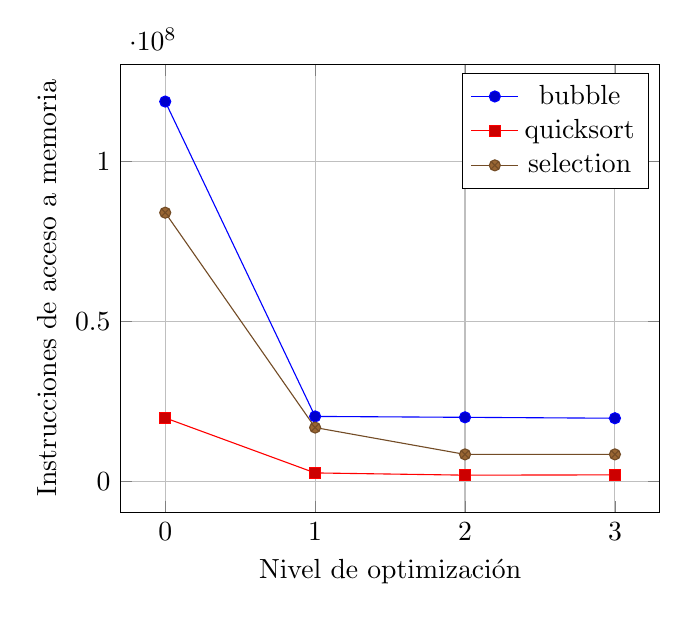
\begin{tikzpicture}
\begin{axis}[
xlabel=Nivel de optimización,
ylabel=Instrucciones de acceso a memoria,
grid=major,
xtick=data]
\addplot coordinates {
(0,118828473)
(1,20281490)
(2,19997926)
(3,19714362)
};
\addplot coordinates {
(0,19815975)
(1,2595975)
(2,1897211)
(3,1986973)
};
\addplot coordinates {
(0,84049617)
(1,16797696)
(2,8398848)
(3,8402944)
};
\legend{bubble,quicksort,selection}
\end{axis}
\end{tikzpicture}
\end{center}
\caption{Comparación de instrucciones de acceso a memoria entre funciones y optimizaciones.}
\label{graph:memoria}
\end{figure}

Si nos fijamos en la gráfica de la figura~\ref{graph:memoria}, vemos cómo en el nivel inicial de optimización hay número de accesos a memoria, que puede llegar a suponer alrededor de la mitad de las instrucciones totales de la funcion, reduciendose notablemente en los niveles superiores. Esta diferencia se debe, principalmente, al uso que se hace de los registros disponibles según el nivel de optimización. Por ejemplo, si vemos el código en ensamblador de \orden{bubble0} nos damos cuenta de que solamente hace uso de dos registros durante su ejecución: \orden{v0} y \orden{v1}. Por otro lado, en \orden{bubble1}, \orden{bubble2} y \orden{bubble3} se utilizan, no solo \orden{v0} y \orden{v1} sino también otros registros como \orden{a1}, \orden{a2} y \orden{a3}, aprovechando mejor los recursos disponibles en el procesador.

\begin{figure}[htbp]
\begin{center}
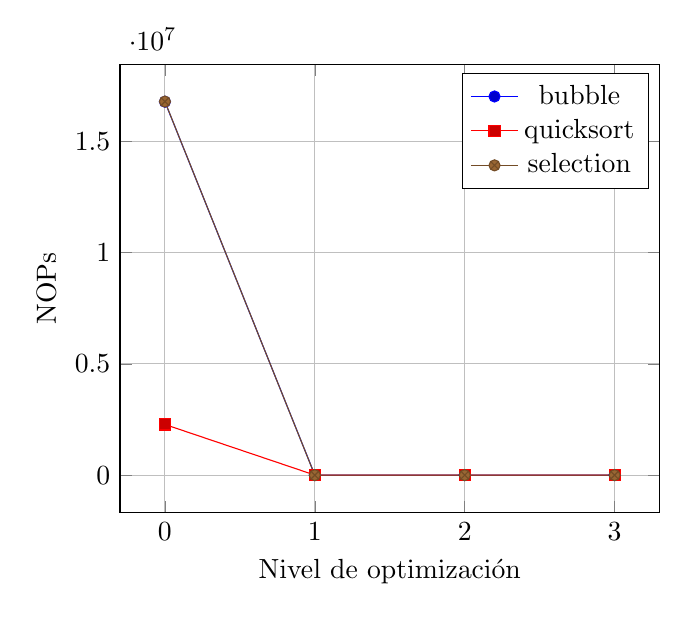
\begin{tikzpicture}
\begin{axis}[
xlabel=Nivel de optimización,
ylabel=NOPs,
grid=major,
xtick=data]
\addplot coordinates {
(0,16785411)
(1,4097)
(2,4097)
(3,4097)
};
\addplot coordinates {
(0,2278408)
(1,3403)
(2,0)
(3,0)
};
\addplot coordinates {
(0,16793603)
(1,1)
(2,1)
(3,1)
};
\legend{bubble,quicksort,selection}
\end{axis}
\end{tikzpicture}
\end{center}
\caption{Comparación de instrucciones \orden{nop} entre funciones y optimizaciones.}
\label{graph:nops}
\end{figure}
El número de instrucciones \orden{nop}, como se aprecia en la figura~\ref{graph:nops}, es considerablemente alto en las funciones cuyo nivel de optimización es `0', pero se reduce en el resto de los niveles de optimización, con respecto al más bajo. La cantidad de \orden{nop} en una función nos da una idea de la eficencia de la misma, ya que esta instrucción supone que el procesador no comienza una instrucción nueva en ese ciclo. El número es alto en el nivel inferior de optimización ya que el compilador no trata de reordenar las funciones para evitar dependencias entre ellas, lo que supone que el procesador deba esperar a que esté el dato disponible o a poder usar la unidad aritmético-lógica. Muchos de estos ciclos de espera también se producen después de las instrucciones de salto, en las funciones sin optimizar. Esto se debe a que no se puede realizar el salto hasta que no se haya calculado la dirección a la que se ha de ir, de ahí el \orden{nop} que podemos ver en el código desensamblado de todas las funciones sin optimizar detrás de este tipo de instrucciones. En los siguientes niveles, se aprovecha este espacio para colocar ahí una instrucción anterior a la de salto, siempre y cuando el resultado de esta función no sea determinante para calcular la dirección de destino del propio salto.

\subsection{Depuración y legibilidad del código.} % (fold)
\label{sub:Depuración y legibilidad del código.}
A partir del primer nivel de optimización el tamaño de la función y los tipos de instrucciones en ensamblador que podemos encontrar no varían mucho. Sin embargo sí que se producen reordenamiento de las instrucciones por parte del compilador para aprovechar mejor las unidades funcionales del microprocesador. Esto tiene la desventaja de que, a la hora de depurar el código ensamblado, es más difícil relacionar las instrucciones en lenguaje MIPS con las correspondientes en C.\@ Por ello, durante la fase de desarrollo del programa se debe mantener el nivel de optimización más bajo posible para facilitar la tarea de depuración.

Esto se puede observar en las funciones desensambladas del apéndice~\ref{chap:apendice4}. Por ejemplo, en las funciones que han sido compiladas usando el nivel de optimización `0', detrás de las instrucciónes de salto condicional siempre encontramos un \orden{nop}. Sin embargo, en el resto, debido a la opción \orden{-fdelayed-branch} encontramos en su lugar instrucciones que se ejecutarían antes si no se hubiese usado esta opción. Lo que puede dar lugar a confusión cuando se revisa el código (sobre todo si no se está familiarizado con estas optimizaciones y el modelo de programación de MIPS).

La desventaja de leer y depurar el código compilado sin optimizaciones es el exceso de movimientos entre el stack y los registros que se producen. Si acudimos otra vez al ejemplo de la función \orden{bubble0}, se puede ver cómo, durante toda la función, se guardan continuamente los valores de los registros \orden{v0} y \orden{v1} en el stack y, a continuación, se vuelven a leer. Esto no ocurre en el resto de funciones ya que en estas se hace más uso de los registros y menos del stack.
% subsection Depuración y legibilidad del código. (end)

\section{Análisis del tiempo de ejecución.} % (fold)
\label{sec:Análisis del tiempo de ejecución.}
Ya hemos visto el aspecto de las funciones en ensamblador, la cantidad de instrucciones en cada una de ellas y el tipo de instrucciones que las componen. Pero, ¿cómo se traducen estas diferencias en el rendimiento final de la aplicación? ¿hasta qué punto merece la pena el aumento de la complejidad del código ensamblador?.

Normalmente, el nivel de optimización con el que se compila un programa también afecta al propio tiempo de compilación del mismo. Debido al tamaño del programa del que aquí se trata (el archivo del programa del apartado anterior que se carga a la placa ocupa solamente 314~kB y su compilación tarda 3 segundos en mi portátil), este hecho se obvia al no tener un gran impacto en el proceso de creación de un programa para Chipkit o Arduino.

Hay varias formas de determinar el rendimiento de un programa o función. Podemos, por ejemplo, medir cuántos cálculos realiza por unidad de tiempo, pero esta medida no es adecuada para el este tipo de aplicación. En este caso lo que se intenta conseguir (en términos de rendimiento y optimización) es reducir el retardo que se produce desde que el usuario envía la órden hasta que obtiene la respuesta. Por lo que para saber el rendimiento de cada función y nivel de optimización, se usará el tiempo que tarda en ejecutarse dicha función, que será el tiempo de respuesta de la aplicación~\footnote{Cuando se ejecuta una órden este debe ser procesado, al igual que el vector de números que se pasa como parámetro, pero este tiempo será constante en todas las funciones al ser su código común a todas ellas.}.

\begin{figure}[htbp]
\begin{center}
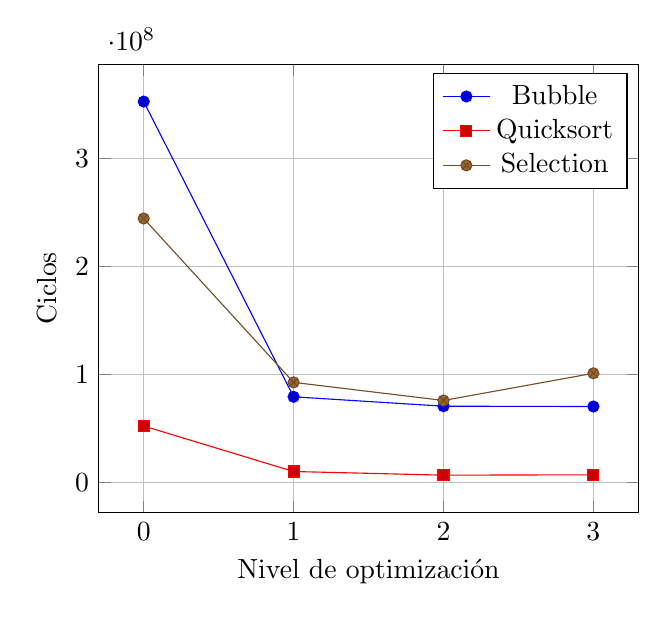
\begin{tikzpicture}
\begin{axis}[
xlabel=Nivel de optimización,
ylabel=Ciclos,
grid=major,
xtick=data]
\addplot coordinates {
	(0,352390396)
	(1,79200250)
	(2,70509212)
	(3,70225162)
};
\addplot coordinates {
	(0,	52175666)
	(1,	10090462)
	(2,	6713156)
	(3,	7025934)
};
\addplot coordinates {
	(0,	244191650)
	(1,	92569958)
	(2,	75805786)
	(3,	100967950)
};
\legend{Bubble,Quicksort,Selection}
\end{axis}
\end{tikzpicture}
\end{center}
\caption{Número de ciclos según función y optimización}
\label{graph:ciclos}
\end{figure}

En la figura~\ref{graph:ciclos} están representados la cantidad de ciclos de procesador que ha llevado ejecutar cada una de las funciones según el nivel de optimización. Se observa un patrón claro, al reducirse el tiempo de ejecución considerablemente cuando se utiliza el primer nivel de optimización, con respecto al inicial. Por ejemplo en el caso del algoritmo `Quick Sort' esta reducción supone un 80\% menos de ciclos tan solo eligiendo el primer nivel de optimización, siendo menor en los otros dos. Incluso en el nivel de optimización `0', este algoritmo ya es más rápido que cualquiera de los otros dos en el tercer nivel de optimización.

Si nos fijamos en la ganancia de rendimiento para niveles de optimización más altos que el primero, se puede ver que es muy inferior a la que se obtiene con el primer nivel (en comparación al nivel `0'). Este resultado es de esperar debido a que las optimizaciones que se llevan a cabo en los niveles superiores son más específicas y en estos algoritmos no tienen gran efecto. En el caso del algoritmo de selección, además, vemos como, no solo no se reduce el tiempo de ejecución al usar el tercer nivel de optimización, sino que aumenta con respecto al primer y segundo nivel. Este comportamiento no lo vemos en las otras funciones que, aunque muy limitada, si presentan una ganancia en el rendimiento final.
\begin{table}[htb]
	\begin{center}
		\begin{tabular}{lllll}
      \textbf{Algoritmo} & \textbf{Nivel 0} & \textbf{Nivel 1} & \textbf{Nivel 2} & \textbf{Nivel 3} \\
      \hline
      \textit{Bubble		}&	352390396	&	79200250 (77.52\%)	&	70509212 (10.97\%)	&	70225162 (0.4\%) \\
			\textit{QuickSort	}	&	52175666	&	10090462	(80.66\%)	&	6713156 (33.47\%)	&	7025934 (-4.66\%) \\
			\textit{Selection	} &	244191650	&	92569958 (62.09\%)	&	75805786 (18.11\%)	&	1009679 (-33.19\%) \\
		\end{tabular}
	\end{center}
\caption{Algoritmos y ciclos de ejecución. Ganancia con respecto al nivel anterior entre paréntesis.}
\label{tabla:ciclos}
\end{table}
% section Análisis del tiempo de ejecución. (end)
\section{Limitaciones de la biblioteca Arduino.} % (fold)
\label{sec:Limitaciones de la biblioteca Arduino.}

La plataforma Arduino, incluyendo Chipkit, está pensada para poder crear programas sin tener que conocer el funcionamiento interno de cada microcontrolador. Es una capa de abstracción más, que permite usar las mismas funciones o incluso programas en microcontroladores diferentes. Por ejemplo, si ejecutamos la función \orden{digitalWrite(13, HIGH)} sabemos que se encenderá el LED de usuario que tienen instalado todas las placas convencionales compatibles con Arduino. No es necesario conocer a que puerto del microcontrolador está conectado dicho LED, que varía según el modelo de placa. Por ejemplo, en el chipKIT MAX32 este LED (LD4) se encuentra conectado al tercer pin del puerto A, sin embargo, en el chipKIT Uno32 lo encontramos el el sexto pin del puerto G.\@

Cuando queremos leer un valor en una de las entradas analógicas ocurre algo similar: a la función \orden{analogRead()} solo hay que pasarle el pin de la placa, cuyo número se encuentra impreso al lado del mismo y la función se encarga de realizar toda la configuración necesaria para obtener el valor del ADC.\@

Esta simplificación tiene un precio. Cada vez que se quiere leer o escribir en cada uno de estos puertos, la función encargada de hacerlo lleva a cabo la configuración y la posterior lectura o escritura. Esta sobrecarga hace que cualquiera de estas operaciones sea considerablemente más lenta que si se realizara con funciones de más bajo nivel o accediendo directamente a los registros.

Para ilustrar la diferencia he medido de dos formas distintas la frequencia a la que es capaz el Chipkit Max32 de cambiar el estado de un pin de salida. Usando la funcion de Arduino para escribir en una salida digital (\orden{digitalWrite()}) y accediendo a los registros directamente he generado dos ondas cuadradas de diferentes frecuencias. La primera forma de medir la diferencia ha sido usando un método similar al que usamos en el apartado anterior: guardando el valor del contador del microprocesador antes y después de la ejecución de lo que se desea medir. En este caso he optado por medir el tiempo que tarda en ejecutarse un bucle `for' en el que se pone a alto y bajo un pin del microcontrolador. El bucle se repite \(10^5\) veces.

\begin{table}[htb]
	\begin{center}
		\begin{tabular}{llllll}
      \textbf{Método}		&		\textbf{Cuentas}		&		\textbf{Ciclos}		&		\textbf{Ciclos/iteración}	&		\textbf{Periodo}		&		\textbf{Frecuencia} \\
			\hline
      \textit{Arduino}		&		5763684		&		11527368	&		115.27						&		1.44 us		&		694 kHz \\
      \textit{Registros}	&		501040		&		1002080		&		10.02							&		125.26 ns	&		7.98 MHz \\

		\end{tabular}
	\end{center}
	\caption{Diferencia entre \orden{digitalWrite()} y acceso directo al registro usando un bucle \orden{for} de $10^5$ iteraciones y midendo el tiempo que tarda en completarse este bucle.}
	\label{ard_vs_reg:1}
\end{table}

En la figura~\ref{ard_vs_reg:1} se puede apreciar la diferencia de velocidad cuando se realiza la escritura digital en un puerto dependiendo del método empleado. Según estos datos el acceso directo a los registros del microcontrolador nos otorga la posibilidad de ejecutar esta operación a una frecuencia un orden de magnitud mayor que con la función \orden{digitalWrite()} de la biblioteca Arduino. Para contrastar los resultados también he obtado por realizar las mediciones con otro método. Usando un bucle infinito con \orden{while(1)} he medido la frecuencia de la onda cuadrada que se genera en el pin correspondiente y, como se puede ver en la figura~\ref{ard_vs_reg:2} los resultados son muy similares al primer método.

\begin{table}[htb]
	\begin{center}
		\begin{tabular}{ll}
      \textbf{Método}		&		\textbf{Frecuencia}	\\
			\hline
      \textit{Arduino}		&		700 kHz			\\
      \textit{Registros}	&		7.983	MHz		\\
		\end{tabular}
	\end{center}
	\caption{Frecuencia de conmutación según el método empleado. Medida usando un multímetro UNI-T UT61E}
	\label{ard_vs_reg:2}
\end{table}

Esta diferencia de velocidad dependiendo del método empleado es debida a que las funciones de la biblioteca Arduino no se encargan solo de, por ejemplo, escribir en un pin digital, también comprueban que el pin existe y en el caso de existir, a que puerto del microcontrolador pertenece. Como el objetivo de la biblioteca Arduino no es solo simplificar funciones comunes en microcontroladores, sino también generar código portable, es decir, código que pueda ser compilado en diferentes microcontroladores, las funciones deben ser capaces de ejecutarse teniendo en cuenta esto. Cuando usamos registros la velocidad aumenta, como ya he dicho, a expensas de reducir la legibilidad del código y su portabilidad.

Otra limitación de Arduino es la falta de funciones para controlar características de cada microcontrolador, como por ejemplo interrupciones y temporizadores. Si queremos hacer uso de alguna de estas características no queda más remedio que acudir a las funciones del fabricante o directamente a los registros del microcontrolador. Otro ejemplo de este tipo de limitación está presente en el programa escrito para la siguiente sección. En este programa se muestrea de forma regular (a 8 kHz) una entrada analógica. Esto no es posible realizarlo con la función de Arduino \orden{analogRead()} ya que es demasiado lenta, al tener que configurar cada vez el pin de entrada. Usando los registros del microcontrolador podemos configurar el ADC para que tome muestras de forma regular~\footnote{En el caso del chip que incorpora el Chipkit Max32 se pueden alcanzar frecuencias de muestreo de 1 Msps.} y autónoma, generando una interrupción cuando la muestra está lista.
% section Limitaciones de la biblioteca Arduino. (end)

\section{Ejemplo de aplicación relacionada con la carrera de telecomunicación.} % (fold)
\label{sec:Ejemplo de aplicación relacionada con la carrera de telecomunicación.}
% section Ejemplo de aplicación relacionada con la carrera de telecomunicación. (end)

Para finalizar, he decidido escribir una aplicación relacionada con el área de las telecumicaciones. He optado por recrear un programa que elaboré como trabajo final en la asignatura `Laboratorio de tratamiento digital de la señal'. Se trata de un detector de tonos mediante el uso del algoritmo de Goertzel. El programa que desarrollé durante la asignatura funcionaba en un DSP, más concretamente se trataba de un Analog Devices ADSP-2181~\footnote{www.analog.com/en/processors-dsp/adsp-21xx/adsp-2181/products/product.html}.
\begin{figure}[htb]
\centering
\begin{tikzpicture}
	\matrix[row sep=15mm, column sep=25mm]
	{
		\node[dspnodeopen,dsp/label=left]	(m00)	{$x[n]$};	&
		\node[dspadder]						(m01)	{};			&
		\node[dspnodeopen]					(m02)	{$v_k[n]$}; &
		\node[dspadder]						(m03)	{};			&
		\node[dspnodeopen,dsp/label=right]	(m04)	{$y[n]$}; 	\\

		\node[coordinate]					(m10)	{};			&
		\node[dspadder]						(m11)	{};			&
		\node[coordinate]					(m12)	{};			&
		\node[coordinate]					(m13)	{};			\\

		\node[coordinate]					(m20)	{};			&
		\node[coordinate]					(m21)	{};			&
		\node[coordinate]					(m22)	{};			\\
	};

	\foreach \i [evaluate = \i as \j using int(\i+1)] in {0,1,2,3}
		\draw[dspflow] (m0\i) -- (m0\j);

	\draw[dspflow] (m11) -- (m01);
	\draw[dspflow] (m02) -- node[midway,right] {$\z^{-1}$} (m12);
	\draw[dspflow] (m12) -- node[midway,above] {$2cos(2\pi{}k/N)$} (m11);
	\draw[dspflow] (m12) -- node[midway,below] {$-W_{n^{k}}$} (m13);
	\draw[dspflow] (m13) -- (m03);
	
	\draw[dspflow] (m12) -- node[midway,right] {$\z^{-1}$} (m22);
	\draw[dspflow] (m22) -- node[midway,above] {$-1$} (m21);
	\draw[dspflow] (m21) -- (m11);

\end{tikzpicture}
\caption{Algoritmo de Goertzel.}
\label{goertzel}
\end{figure}

El DSP tomaba muestras con una frecuencia de muestreo de 8 kHz, que es la misma que he usado en este programa. Normalmente un DSP toma una muestra y realiza el procesado que requiera el algoritmo en dicha muestra. Este programa hace uso de la posibilidad que tienen los ADC de este microcontrolador de realizar el muestreo automáticamente. De esta forma, una vez configurado, solo hay que escribir una función que se encargue de recoger la muestra cuando el ADC genera una interrupción y decidir cuando empieza y acaba el automuestreo. Las funciones que gestionan una interrupción deben ser lo más cortas posibles, por lo que en las primeras revisiones del programa, esta función se encargaba solomente de almacenar la muestra en un vector y aumentar el contador de muestras. Una vez estan todas las muestras almacenadas, se para el automuestreo y comienza el procesado de los datos en la función \orden{loop()}. Cabe mencionar que este muestreo automático y regular no es posible implementarlo usando tan solo las funciones de la biblioteca Arduino, por lo que es necesario recurrir al manual del microcontrolador y a sus registros para llevarlo a cabo.

Este programa toma las muestras a la misma frecuencia que el DSP de prácticas~\footnote{Aunque, de acuerdo a las especificaciones del PIC32MX795F512L, es capaz de alcanzar frecuencias de muestreo de 1 MHz.}. Viendo el número de operaciones y su complejidad decidí implementarlas directamente en la función de interrupción del ADC, al haber tiempo suficiente entre interrupciones para realizar las operaciones que requiere cada muestra. Con esto logré un funcionamiento idéntico al programa del DSP.\@

Durante las primeras revisiones del programa, todas las operaciones matemáticas que el algoritmo requiere se realizaban usando variables de tipo \orden{float}, es decir, de coma flotante. Como ya comenté en el apartado dedicado al PIC32MX795F512L, este chip no dispone de unidad de coma flotante. Como consecuencia, todas las operaciones sobre variables de este tipo deben ser emuladas mediante el uso de una biblioteca. Realizar las operaciones de este modo consume muchos ciclos del procesador, lo que imposibilitaba el mover las operaciones que se realizaban en cada muestra a la función que gestiona las interrupciones.

Para aumentar la velocidad del programa, decidí usar coma fija. Debido a la naturaleza de las muestras obté por representar con 16 bits el rango de -1 a 1 que, convertido a este formato sería -32767 a 32767 (\(-2^{15}+1\) a \(2^{15}-1\)). Con 16 bits tenemos suficiente precisión ya que las muestras que toma el ADC son de 10 bits y además tenemos la posibilidad de multiplicar dos de estos números y obtener uno de 32 bits que, al ser este el tamaño de palabra del procesador, las operaciones no requeriran más de un ciclo. Para convertir los datos del ADC a esta representación tan solo hace falta realizar un desplazamiento, al igual que para reducir los números de 32 bits a 16. La ventaja de esto en lugar de haber multiplicado por una potencia de 10 los números es que los desplazamientos se ejecutan en un ciclo.

% Goertzel y Filtros Digitales
% Muestreo
% Procesamiento de cada muestra y procesamiento final

\subsubsection{Análisis de rendimiento}

A grandes rasgos, podemos dividir el funcionamiento del programa en dos partes: la recursiva y una parte final. En este caso la parte recursiva del programa es el procesamiento que se realiza de cada muestra recogida y convertida por el ADC del microcontrolador. La frecuencia de muestreo se verá principalmente limitada por este procesamiento de cada muestra, ya que he elegido realizarlo nada más obtenerla para imitar lo mas fielmente posible el funcionamiento de un DSP\@. Como alternativa, se pueden guardar todas las muestras en un vector y, una vez llenado, iterar sobre este realizando el procesado de todas las muestras.

Cada uno de los dos métodos tiene sus ventajas. Si optamos por usar el primero, de forma similar a un DSP, el tiempo en el que se obtiene un resultado al finalizar el muestreo será menor, suponiendo que la frecuencia de muestreo sea tal que permita el correcto procesamiento de cada muestra entre muestreos. La ventaja del segundo método es que, al no tener que realizar el procesamiento entre muestreos podemos reducir el tiempo entre ellos y por lo tanto aumentar su frecuencia, lo que en este caso nos permitiría, por ejemplo, detectar frecuencias mayores al primer método.

\begin{minipage}{\linewidth}
\begin{lstlisting}
extern "C"
{
  void __ISR(_ADC_VECTOR, ipl6) ADCInterruptHandler()
  {
    IFS1CLR = 2;
    /* Normaliza la muestra y la atenua para evitar la saturacion
       al final del filtro. */
    int muestra = ADC1BUF0;
    muestra = muestra - 512;
    muestra = muestra << (GAIN_BITS - 9);
    muestra *= ATENUADOR;
    muestra >>= GAIN_BITS;
    
    /* Guardamos el valor maximo de las muestras */
    if(abs(muestra) > abs(max)) {
      max = muestra;
    }

    /* Parte recursiva de Goertzel */
    q0 = (COSENO * q1);
    q0 -= (MITAD * q2);
    q0 += (COSENO * q1);
    q0 -= (MITAD * q2);
    q0 >>= GAIN_BITS;
    q0 += muestra;
    q2 = q1;
    q1 = q0;

    /* Aumentamos el valor del contador de muestras */
    contador_muestras++;

    /* Si tenemos todas las muestras, cancelamos el
       automuestreo para llevar a cabo la parte 
       final del algoritmo */
    if(contador_muestras >= N_MUESTRAS)
    {
      contador_muestras = 0;
      muestras_listas = true;
      AD1CON1bits.ASAM = 0; // Paramos el automuestreo
    }
  }
}
\end{lstlisting}
\end{minipage}

Este código es el que se ejecuta cada vez que el ADC ha terminado de convertir una muestra~\footnote{El microcontrolador está configurado para que realice el muestreo y la conversión de forma automática con una frecuencia de 8kHz, interrumpiendo cuando se haya completado.}, por lo que es la parte que más interesa analizar para conocer el rendimiento final. Se puede dividir en aproximadamente tres partes. En la primera se obtiene el valor guardado en el registro del ADC, se normaliza, se le aplica una atenuación para evitar saturar el filtro y se guarda el valor máximo para compararlo al final con el valor que devuelve el algoritmo. En la segunda parte se realiza la parte recursiva del algoritmo sobre la muestra actual. Por último, se controla la cantidad de muestras que se han procesado y, en el caso de estar todas, se para el automuestreo para comenzar el procesamiento final en la parte principal del programa.

\begin{figure}[htb]
  \begin{minipage}{.45\textwidth}
\begin{lstlisting}[language={[mips]Assembler},basicstyle=\ttfamily\scriptsize]
 0:	415de800  rdpgpr	sp,sp
 4:	401a7000  mfc0	k0,c0_epc
 8:	401b6000  mfc0	k1,c0_status
 c:	27bdffe8  addiu	sp,sp,-24
10:	afbb0010  sw	k1,16(sp)
14:	7c1b7844  ins	k1,zero,0x1,0xf
18:	377b1800  ori	k1,k1,0x1800
1c:	afba0014  sw	k0,20(sp)
20:	409b6000  mtc0	k1,c0_status
24:	afa30008  sw	v1,8(sp)
28:	afa20004  sw	v0,4(sp)
2c:	24030002  li	v1,2
30:	3c020000  lui	v0,0x0
34:	ac430000  sw	v1,0(v0)
38:	97820000  lhu	v0,0(gp)
3c:	3c030000  lui	v1,0x0
40:	8c630000  lw	v1,0(v1)
44:	afa4000c  sw	a0,12(sp)
48:	3042ffff  andi	v0,v0,0xffff
4c:	3c040000  lui	a0,0x0
50:	00021080  sll	v0,v0,0x2
54:	24840000  addiu	a0,a0,0
58:	00441021  addu	v0,v0,a0
5c:	ac430000  sw	v1,0(v0)
60:	3c020000  lui	v0,0x0
64:	24030004  li	v1,4
68:	ac430000  sw	v1,0(v0)
\end{lstlisting}
\end{minipage}
\hfill
\begin{minipage}{.45\textwidth}
\begin{lstlisting}[language={[mips]Assembler},basicstyle=\ttfamily\scriptsize]
6c:	97820000  lhu	v0,0(gp)
70:	24420001  addiu	v0,v0,1
74:	3042ffff  andi	v0,v0,0xffff
78:	a7820000  sh	v0,0(gp)
7c:	97820000  lhu	v0,0(gp)
80:	3042ffff  andi	v0,v0,0xffff
84:	2c4212ca  sltiu	v0,v0,4810
88:	14400007  bnez	v0,a8
8c:	24030001  li	v1,1
90:	a7800000  sh	zero,0(gp)
94:	3c020000  lui	v0,0x0
98:	a3830000  sb	v1,0(gp)
9c:	8c430000  lw	v1,0(v0)
a0:	7c031084  ins	v1,zero,0x2,0x1
a4:	ac430000  sw	v1,0(v0)
a8:	8fa4000c  lw	a0,12(sp)
ac:	8fa30008  lw	v1,8(sp)
b0:	8fa20004  lw	v0,4(sp)
b4:	41606000  di
b8:	000000c0  ehb
bc:	8fba0014  lw	k0,20(sp)
c0:	8fbb0010  lw	k1,16(sp)
c4:	409a7000  mtc0	k0,c0_epc
c8:	27bd0018  addiu	sp,sp,24
cc:	41dde800  wrpgpr	sp,sp
d0:	409b6000  mtc0	k1,c0_status
d4:	42000018  eret
 \end{lstlisting}
 \end{minipage}
 \caption{Parte recursiva de Goertzel desensamblada (Segundo nivel de optimización)}
 \label{goertzel_recursivo_ensamblador}
 \end{figure}
 En la figura~\ref{goertzel_recursivo_ensamblador} se encuentra el código que se muestra antes desensambado usando \programa{pic32-objdump} de la misma forma que he hecho con el código del otro programa. Al igual que en el apartado anterior, he contado el número de instrucciones según el tipo y optimización. Debido a la diferente naturaleza de este programa, en vez de contar el número de instrucciones al finalizar la ejecución, he contado el número en una de las iteraciones intermedias de esta parte, es decir, cuando la última parte se evalúa como falsa y no se ejecuta. En la tabla~\ref{tabla:tiempos_goertzel} se puede observar el número de instrucciones obtenido junto con el tiempo que ha llevado ejecutarlas.

\begin{table}[htb]
	\begin{center}
		\begin{tabular}{llll}
			\textbf{Nivel} & \textbf{Ciclos} & \textbf{Tiempo} & \textbf{Instrucciones} \\
			\hline
			\textit{O0} & 114 & \(1.43\mu s\) & 128 \\
			\textit{O1} & 82 & \(1.03\mu s\) & 101 \\
			\textit{O2} & 82 & \(1.03\mu s\) & 100 \\
			\textit{O3} & 82 & \(1.03\mu s\) & 100 \\
		\end{tabular}
		\caption{Tiempos de ejecución de la parte recursiva del programa}
		\label{tabla:tiempos_goertzel}
	\end{center}
\end{table}

La diferencia entre los distintos niveles de optimización es prácticamente despreciable en este caso. Debido a la frecuencia de muestreo de 8kHz que he usado en el programa para simular el DSP usado en clase, el tiempo que hay disponible entre muestras para realizar procesamiento es suficientemente largo como para que no importe el nivel de optimización elegido, para esta aplicación en particular. Con esta frecuencia disponemos de alrededor de \(125\mu s\) entre muestras, mientras que en el peor de los casos (sin optimización) el procesamiento de la muestra solo tarda \(1.43\mu s\).

De hecho, sería posible ejecutar este algoritmo 8 veces de forma simultánea, es decir, realizar ocho procesados distintos de muestra entre muestreos, de forma que podemos, por ejemplo, calcular el dígito marcado en un teléfono analógico (si conectáramos la salida del teléfono a la entrada analógica del microcontrolador) o de cualquier otro dispositivo que generase código de marcación por tonos. 
